% --------------------------------------
%
% XMEN Lab.
% BlockGuide Template Documentation
%
% --------------------------------------

%----------------
% Packages configuration
%----------------
\documentclass[a4paper]{article}

\usepackage[a4paper, left=2.5cm, right=2cm]{geometry} % A4 paper size and thin margins
\usepackage[table,xcdraw]{xcolor} % Required for specifying custom colours

\definecolor{grey}{rgb}{0.9,0.9,0.9} % Colour of the box surrounding the title
\definecolor{LightBlue}{rgb}{0.69,0.768,0.95} % Colour of the box surrounding the title

\usepackage[utf8]{inputenc} % Required for inputting international characters
\usepackage[T1]{fontenc} % Output font encoding for international characters 
%\usepackage[sfdefault]{ClearSans} % Use the Clear Sans font (sans serif)
\usepackage{XCharter} % Use the XCharter font (serif)
\usepackage{graphicx}
\usepackage{draftwatermark} % adds draft watermark

\SetWatermarkLightness{0.85}
\SetWatermarkText{Confidencial}
\SetWatermarkScale{0.7}

\usepackage[owncaptions]{vhistory}
\usepackage{indentfirst}
\usepackage{longtable}

\usepackage{fancyhdr}
\pagestyle{fancy}
\rhead{\leftmark}
\lhead{Block Guide: AWGN}

\usepackage[portuguese]{babel}
\usepackage{adjustbox}
\usepackage{multirow}
\usepackage{listings}
\usepackage{tikz-timing} % timing diagram (waveforms)

\usepackage{blindtext}

\usepackage{hyperref}

\usepackage[T1]{fontenc}
\usepackage[utf8]{inputenc}


\hypersetup{
    colorlinks=true,
    linkcolor=black,
    filecolor=magenta,      
    urlcolor=black,
    bookmarks=true,
}
                                      

\begin{document}


%----------------
% CAPA
%----------------
\begin{titlepage}

% Figures
\begin{figure}
\centering

\begin{minipage}{0.45\textwidth}
    \centering
    
\includegraphics[width=0.9\textwidth]{images/logo.jpg}
\end{minipage}\hfill
\begin{minipage}{0.45\textwidth}
    \centering
    
\includegraphics[width=0.9\textwidth]{images/logo_virtus.png}
\end{minipage}

\end{figure}

% Block name
\vspace{8cm}
\parbox[t]{0.93\textwidth}{ 
\parbox[t]{0.91\textwidth}{
    \centering
    \fontsize{36pt}{40pt}\selectfont
    \vspace{3cm}
    
    % Configure your block name here (<Block Name>):
    \textbf{Core RISC-V \\
    Block Guide}
    
    \vspace{1.5cm}}
}
\end{titlepage}

% Confidential msg    
\pagebreak
\hspace{0pt}
\vfill
\begin{center}
\hfill\rule{\linewidth}{1pt} \\[4pt]
    Este é um documento \textbf{CONFIDENCIAL} \\
    é vetado qualquer reprodução ou divulgação não autorizada.\\[4pt]
    \hfill\rule{\linewidth}{1pt} \\[4pt]
\end{center}
\vfill
\hspace{0pt}
\pagebreak


%----------------
% VERSÕES
%----------------

\renewcommand \vhAuthorColWidth{.8\hsize}
\renewcommand \vhChangeColWidth{1.2\hsize}
 
\renewcommand{\vhhistoryname}{Histórico de Revisão}
\renewcommand{\vhversionname}{Versão}
\renewcommand{\vhdatename}{Data}
\renewcommand{\vhauthorname}{Autor(es)}
\renewcommand{\vhchangename}{Descrição}
 
\begin{versionhistory}
  \vhEntry{1.0}{25/04/19}{George Camboim}{Versão inicial}
\end{versionhistory}

\newpage
\tableofcontents
\newpage
\listoffigures
\newpage
\listoftables
\newpage

% ajusta contagem tabela
\setcounter{table}{0}

%----------------
% CAPITULOS
%----------------
\section{Introdução}
\label{sec:introdução}
Texto...


\subsection{Convenções}
\label{sub:convenções}
Texto...
\section{ISA RISC-V} % (fold)
\label{sec:isa_riscv}

\begin{figure}[!htb]
  \caption{Diagrama do bloco AWGN.}
  \vspace{0.2cm}
  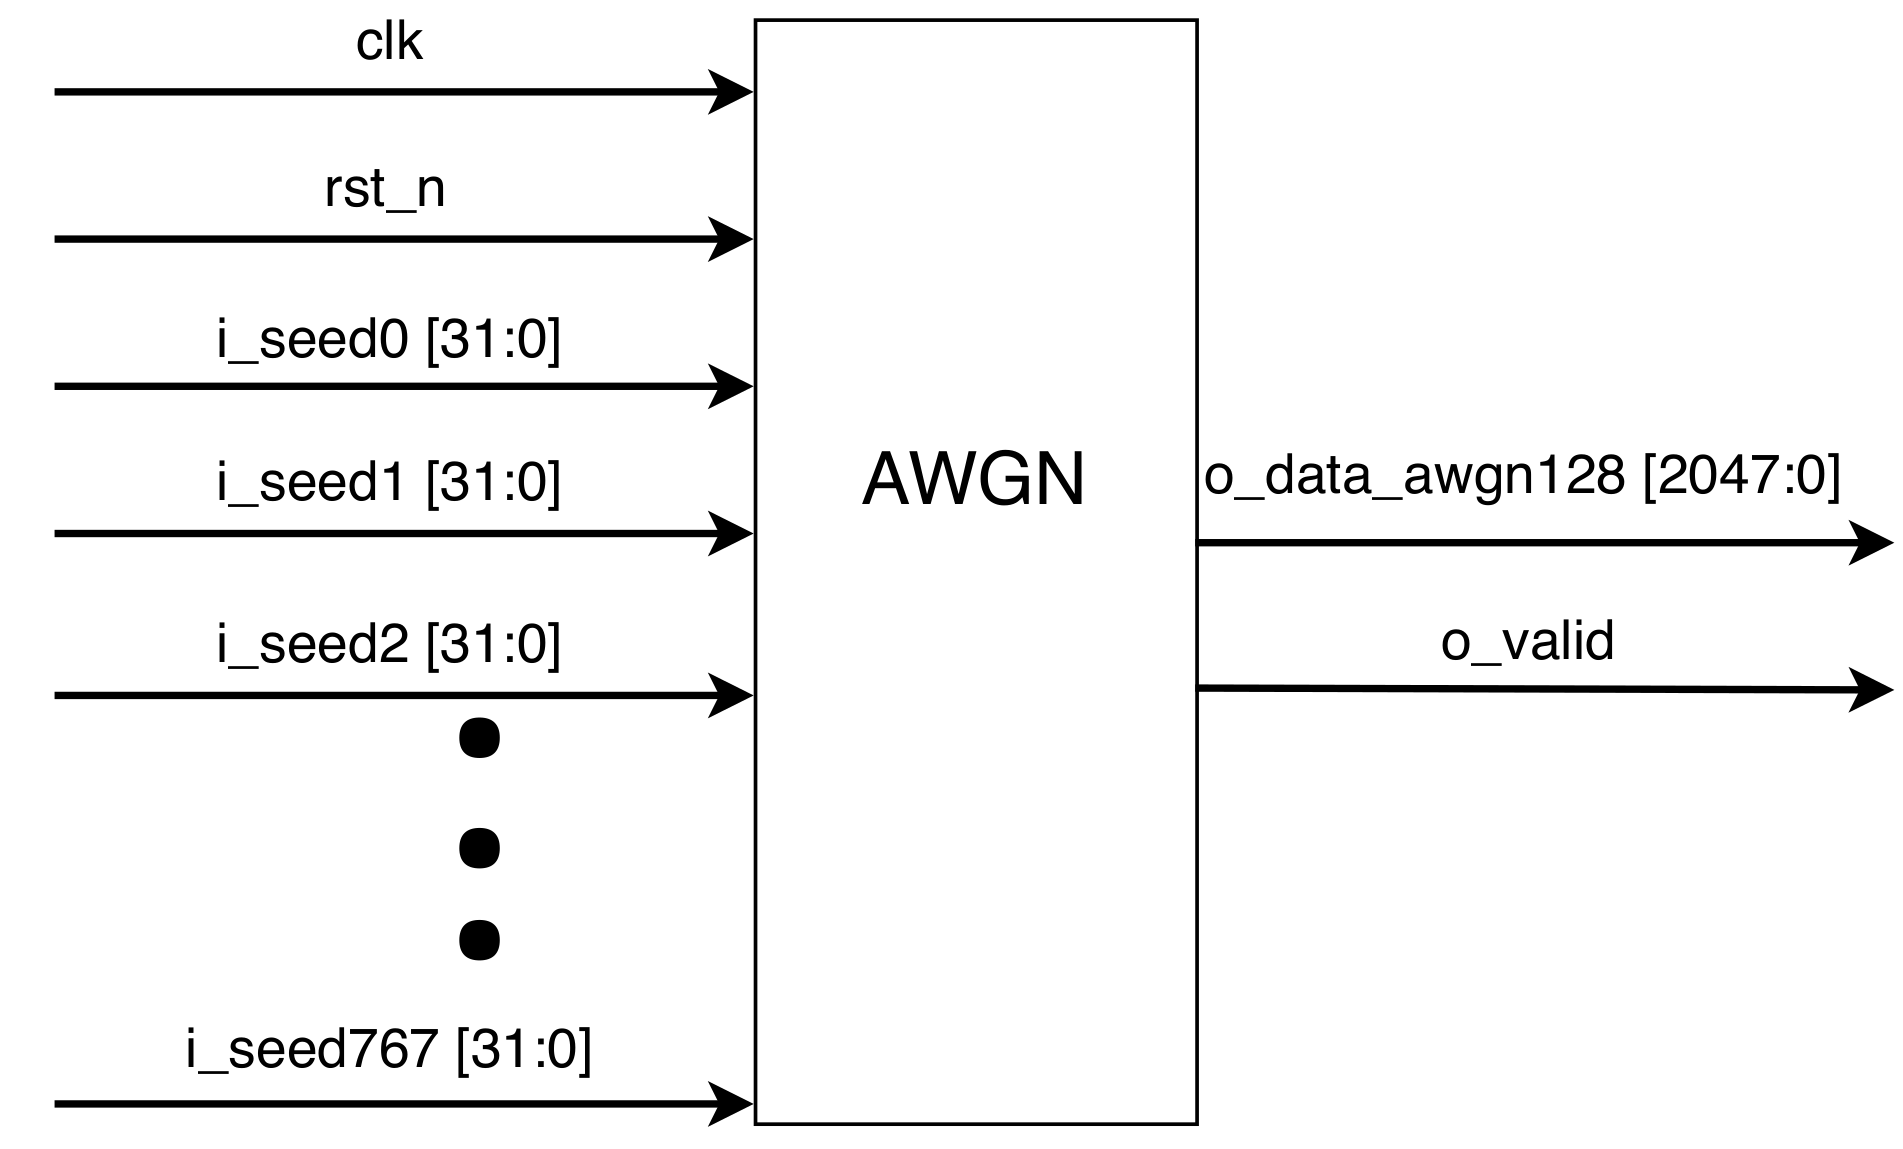
\includegraphics[width=\linewidth]{images/bloco.png}
  \label{fig:top}
\end{figure}

\subsection{Visão Geral}
Texto...

% section introdução (end)

\section{Guia de Blocos} % (fold)
\label{sec:guia_de_blocos}

\begin{itemize}
  \item Não se aplica a esse bloco.

\end{itemize}

\subsection{IF Stage}
\clearpage
\begin{figure}[!htb]
  \caption{Diagrama do bloco IF\_Stage.}
  \vspace{0.2cm}
  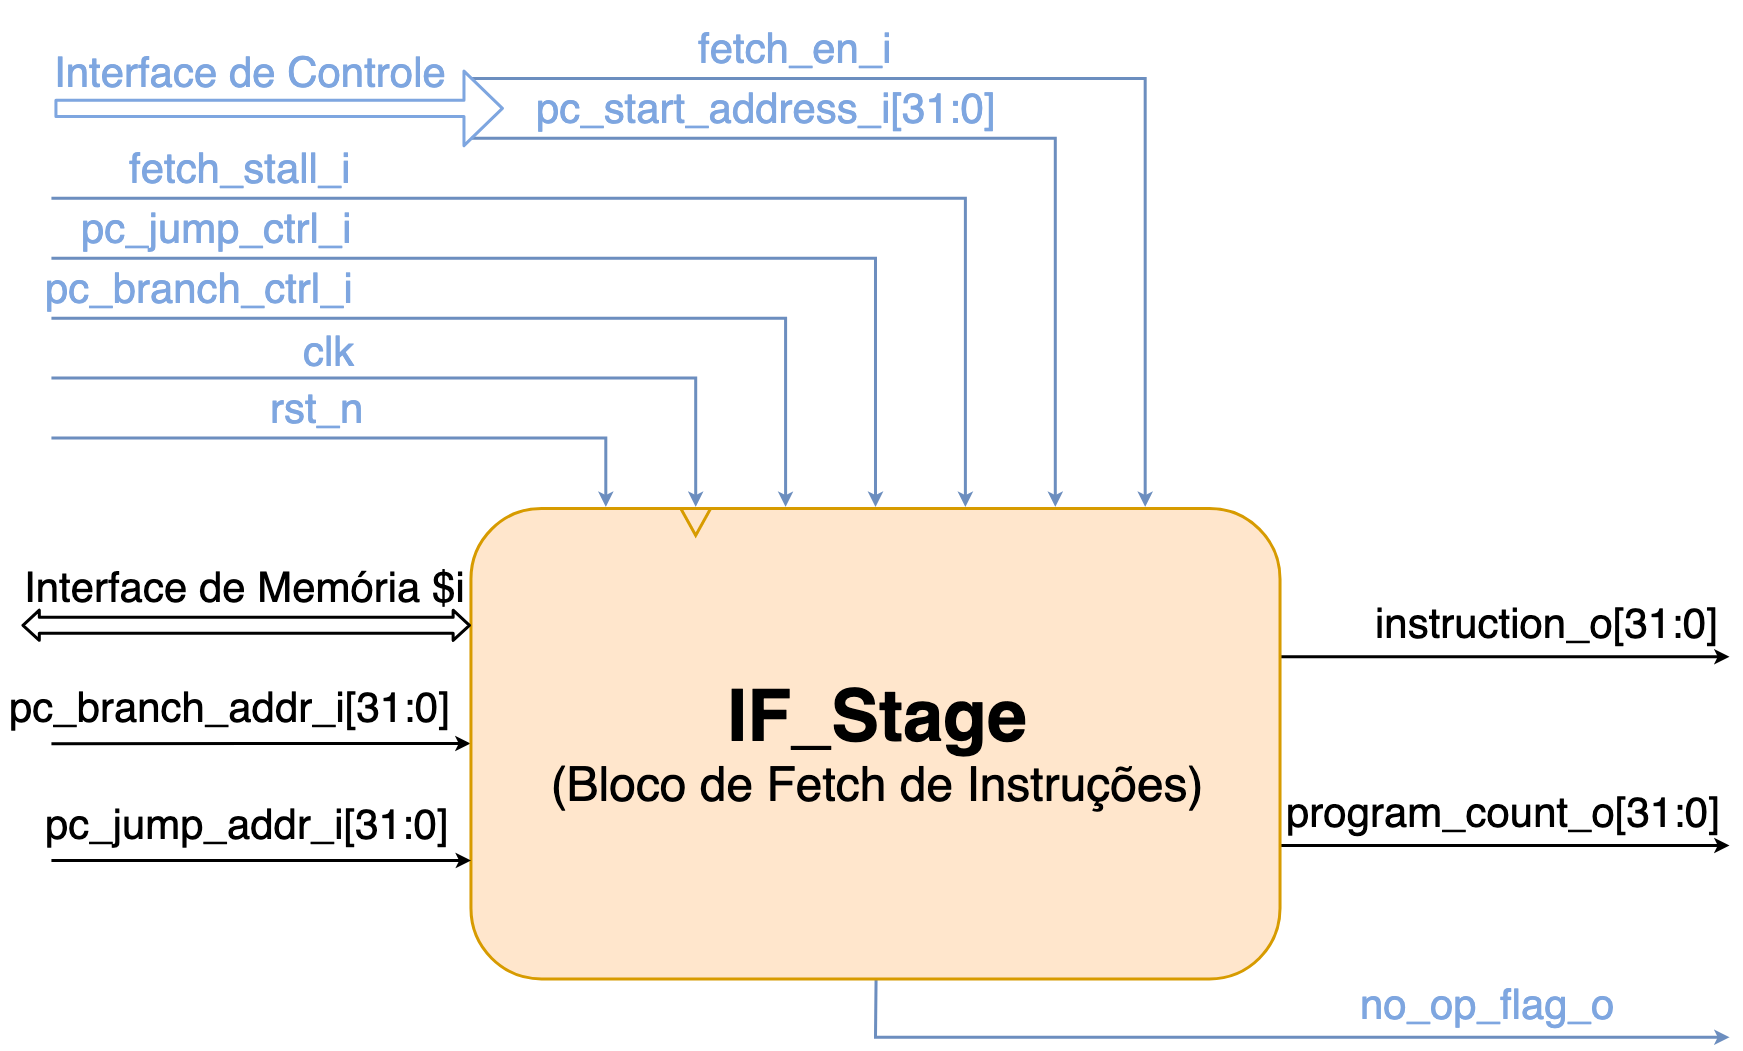
\includegraphics[width=\linewidth]{images/IF_Stage(BLOCK).png}
\end{figure}


\subsection{ID Stage}
\clearpage
\begin{figure}[!htb]
  \caption{Diagrama do bloco AWGN.}
  \vspace{0.2cm}
  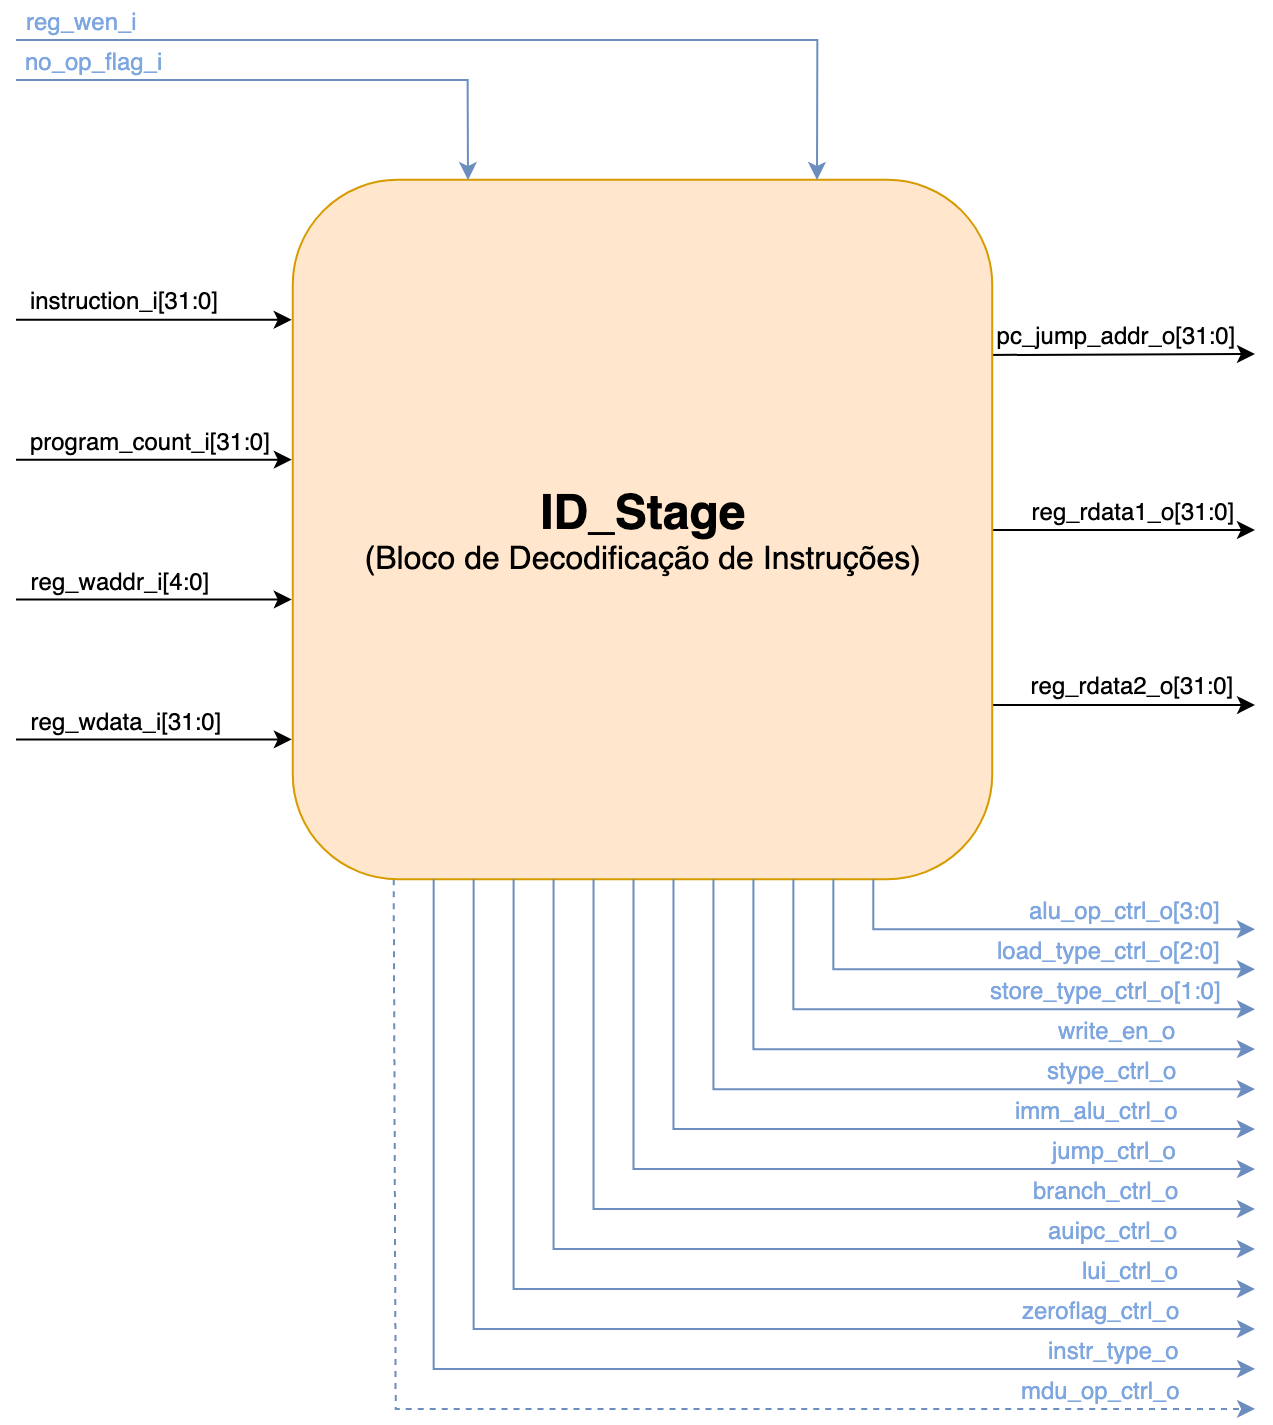
\includegraphics[width=\linewidth]{images/ID_Stage(BLOCK).png}
\end{figure}

\subsection{EX Stage}
\clearpage
\begin{figure}[!htb]
  \caption{Diagrama do bloco AWGN.}
  \vspace{0.2cm}
  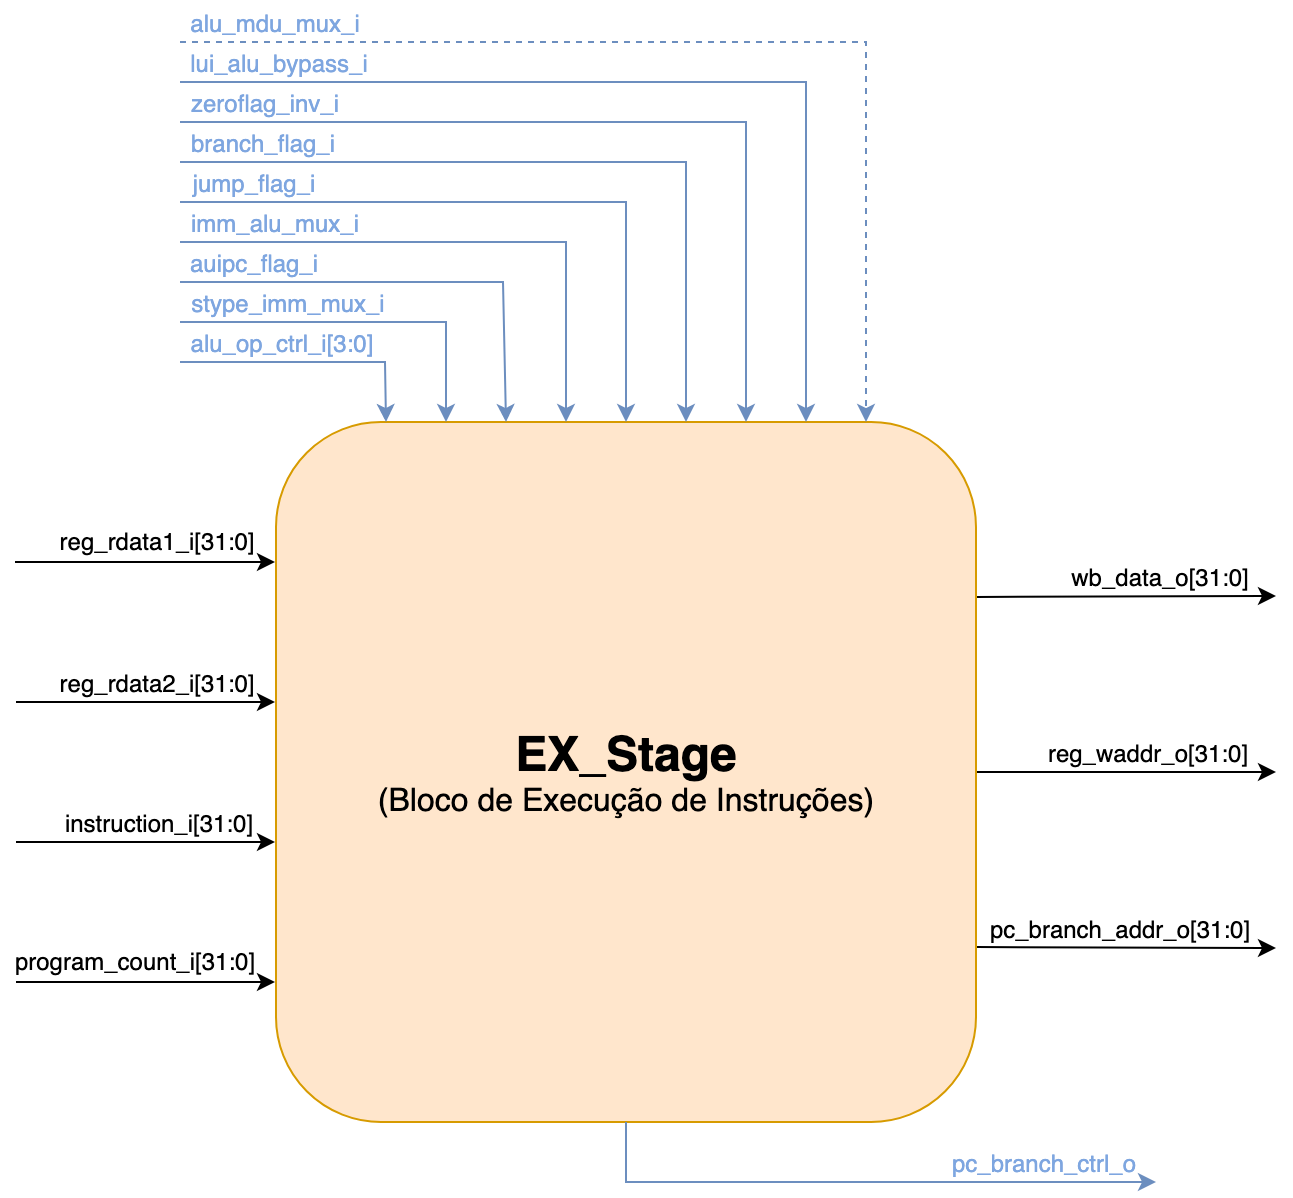
\includegraphics[width=\linewidth]{images/EX_Stage(BLOCK).png}
\end{figure}

\subsection{WB Stage}
\clearpage
\begin{figure}[!htb]
  \caption{Diagrama do bloco AWGN.}
  \vspace{0.2cm}
  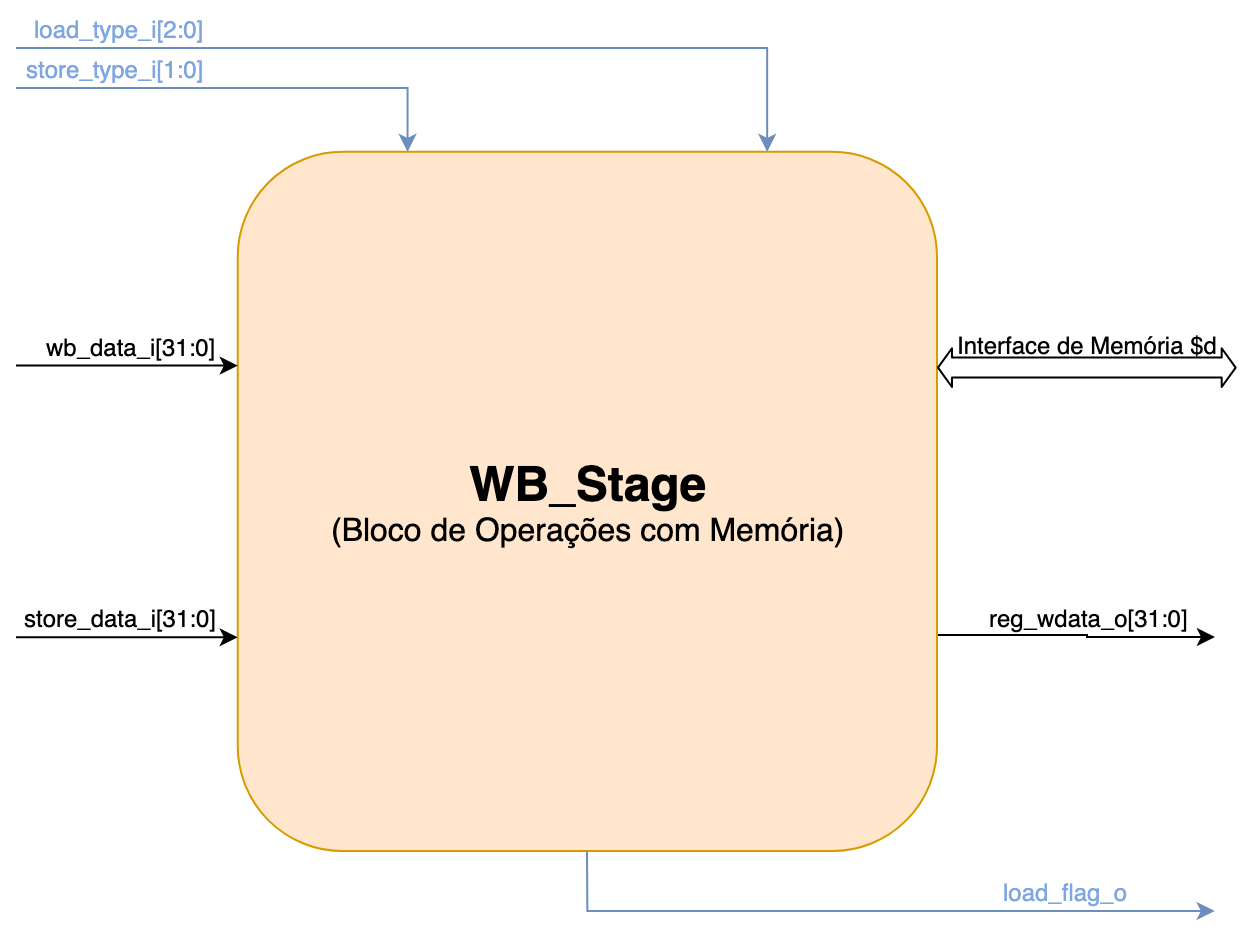
\includegraphics[width=\linewidth]{images/WB_Stage(BLOCK).png}
\end{figure}

\subsection{PCU}


\subsection{Registradores Entre-Estágios}
% subsection descrição_de_registradores (end)

\section{Descrição dos sinais de interfaces} % (fold)
\label{sec:sinais_externos}


\begin{table}[h]
   \centering
   % distancia entre a linha e o texto
    {\renewcommand\arraystretch{1.25}
       \caption{Descrição de sinais}
       \vspace{0.3cm}
        \begin{tabular}{ l l }
         \cline{1-1}\cline{2-2}  
         \multicolumn{1}{|p{3.850cm}|}{\textbf{Convenção} \centering } &
         \multicolumn{1}{p{8cm}|}{\textbf{Descrição} \centering }
           \\  
           \cline{1-1}\cline{2-2}  
          \multicolumn{1}{|p{3.850cm}|}{\vspace{0.3cm} Texto... \centering } &
           \multicolumn{1}{p{8cm}|}{Texto... \centering }
             \\  
             \cline{1-1}\cline{2-2}  
             \multicolumn{1}{|p{3.850cm}|}{\vspace{0.4cm} Texto... \centering } &
             \multicolumn{1}{p{8cm}|}{Texto... \centering }
               \\  
               \cline{1-1}\cline{2-2}  
               \multicolumn{1}{|p{3.850cm}|}{\vspace{0.1cm} Texto... \centering } &
               \multicolumn{1}{p{8cm}|}{Texto... \centering } 
              \\
               \cline{1-1}\cline{2-2}
               \multicolumn{1}{|p{3.850cm}|}{\vspace{0.1cm} Texto... \centering } & 
               \multicolumn{1}{p{8cm}|}{Texto... \centering }
                \\
                   \hline
                   
               \end{tabular}  }
                   \end{table}
% section descrição_detalhada_de_sinais (end)


%----------------
% BIBLIOGRAFIA
%----------------

\end{document}
